\documentclass[12pt,a4paper]{article}

\usepackage[T1]{fontenc}
\usepackage[utf8]{inputenc}
\usepackage[brazil]{babel}
\usepackage{lmodern}
\usepackage{geometry}
\geometry{margin=2.5cm}

\usepackage{amsmath,amssymb}
\usepackage{graphicx}
\usepackage{xcolor}
\usepackage{booktabs}
\usepackage{array}
\usepackage{float}
\usepackage{algorithm}
\usepackage{listings}
\lstdefinestyle{pseudopy}{
  basicstyle=\ttfamily\footnotesize,
  keywordstyle=\bfseries,
  morekeywords={def,for,if,in,return,True,False,break,continue,while,and,or,not,else,append,pop,extend,empty},
  commentstyle=\itshape\color{gray},
  morecomment=[l]{\#},
  showstringspaces=false,
  xleftmargin=1em,
}
\usepackage{tikz}
\usetikzlibrary{arrows.meta,positioning,shapes.geometric,fit,calc}
\usepackage{hyperref}

\hypersetup{
	colorlinks=true,
	linkcolor=blue,
	urlcolor=blue,
	citecolor=blue,
	pdftitle={Segmentação 3D de Órgãos no Ecossistema DocDo},
	pdfauthor={DocDo}
}

\title{Segmentação 3D de Órgãos no Ecossistema DocDo:\\
Dois Algoritmos Práticos para Planejamento Cirúrgico}
\author{Alexandre T. Nogueira}
\date{Maio de 2026}


\begin{document}

\maketitle

\begin{abstract}
O DocDo emprega primariamente dois algoritmos para segmentação 3D de estruturas anatômicas em volumes DICOM pré-processados no 3D Slicer, com mais de dez anos de uso clínico e mais de 1000 pacientes. O primeiro, o \textit{Seeded IFT}~\cite{falcao2004}, realiza expansão de contornos guiada por custo acumulado similar ao algoritmo de Dijkstra, dentro de uma região de interesse delimitada por \textit{bounding box}; o custo local entre voxels é dado pela diferença de intensidade e controlado por \textit{budgets}, \textit{thresholds} e iterações de refinamento. O segundo, o \textit{Orthogonal Vessel Tracker}~\cite{aylward2002}, executa rastreamento vascular por cortes transversais iterativos: busca planos locais de menor área, propaga sementes na direção ortogonal e reconstrói o vaso em 3D por centros e raios locais. Formulações, pseudocódigos e diagramas de fluxo acompanham os dois métodos. Bifurcações vasculares e seções elipsoidais permanecem como limitações abertas.
\end{abstract}

\section{Introdução e motivação clínica}

A segmentação de órgãos e estruturas de interesse em 3D é um passo crítico em um planejamento cirúrgico de cirurgias minimamente invasivas, especialmente quando o procedimento depende de leitura espacial precisa de relações entre tumor, parênquima e vasos. Em cenários reais, essa tarefa precisa equilibrar três dimensões: acurácia anatômica, tempo de execução e controle interativo pelo especialista. No contexto do DocDo, empresa e \textit{software} que fundei, a decisão de engenharia foi priorizar algoritmos robustos e interpretáveis, com forte integração ao fluxo do 3D Slicer, em vez de depender exclusivamente de modelos \textit{black-box}.

Ao longo de cerca de 10 anos, esse pipeline foi aplicado em mais de 1000 pacientes. Porem esse histórico não elimina a necessidade de evolução técnica, mas valida a utilidade prática da estratégia: o médico interage diretamente com o volume, define sementes anatômicas, ajusta parâmetros e exporta geometrias finais (STL) para análise pré-operatória. Com o advento de algoritmos mais sofisticados como CNNs, e modelos de difusão, a base conceitual e operacional desses metodos permanece relevante, porem ainda DocDo ainda nao adotou essas abordagens.

Os dois algoritmos centrais do fluxo são:
\begin{itemize}
	\item \textbf{Seeded IFT}~\cite{falcao2004}: segmentação por expansão com custo acumulado tipo Dijkstra, guiada por sementes em ROI.
	\item \textbf{Orthogonal Vessel Tracker}~\cite{aylward2002}: segmentação e rastreamento de vasos por cortes transversais mínimos iterativos.
\end{itemize}

\section{Visão geral do pipeline no DocDo}

O pipeline segue cinco etapas:
\begin{enumerate}
	\item carregamento do volume DICOM pré-processado;
	\item seleção de uma região-alvo por \textit{bounding box};
	\item marcação de sementes no 3D Slicer;
	\item execução de segmentação (\textit{Seeded IFT} e/ou \textit{Orthogonal Vessel Tracker});
	\item geração de malha e exportação em STL para uso no DocDo.
\end{enumerate}

\begin{figure}[H]
    \centering
    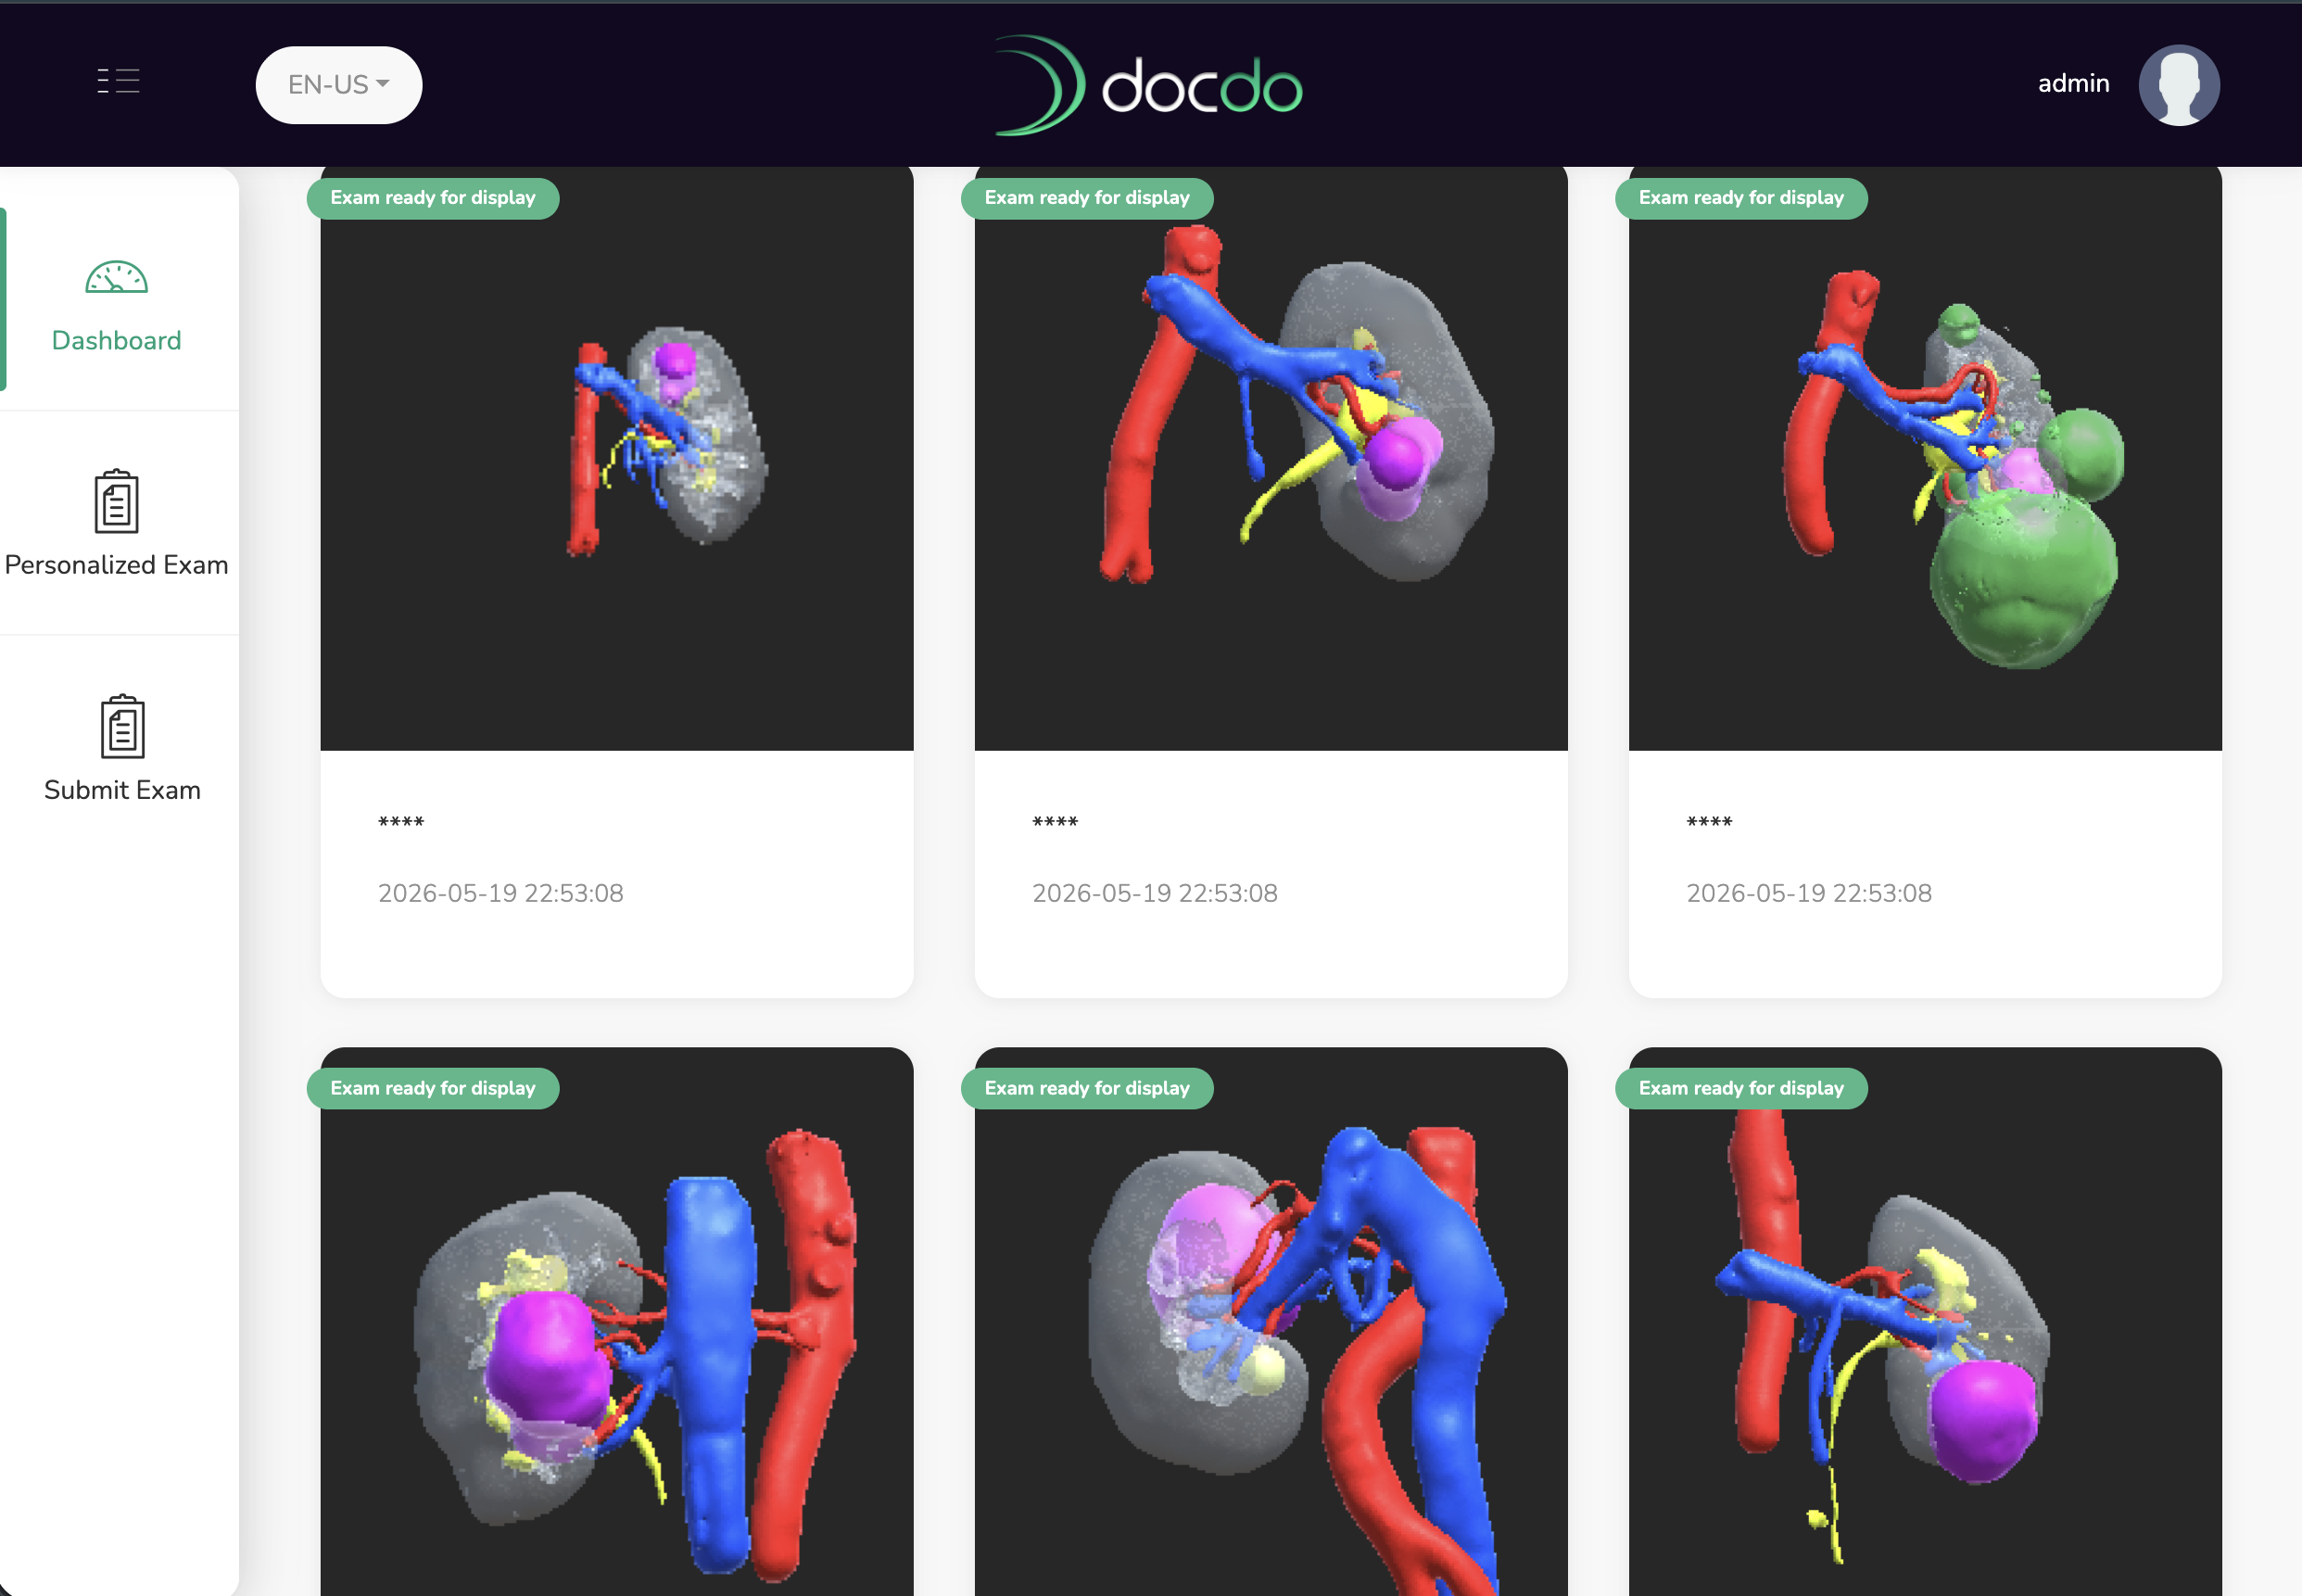
\includegraphics[width=\linewidth]{backoffice}
    \caption{Dashboard do DocDo com seis exemplos reais de reconstrução 3D. Legenda de cores: rim (branco translúcido), artéria renal/aorta (vermelho), veia (azul), tubo coletor/ureter (amarelo), tumores (rosa/roxo) e cistos (verde). Cada caso está pronto para visualização e planejamento cirúrgico interativo.}
    \label{fig:backoffice}
\end{figure}

\section{Seeded IFT: segmentação guiada por sementes com custo acumulado}

\subsection{Intuição}

Dado um volume pré-processado e uma ROI delimitada por \textit{bounding box}, o usuário marca pontos-semente na estrutura alvo. A partir dessas sementes, o algoritmo expande uma frente de busca usando uma fila de prioridade. Cada voxel candidato recebe um custo acumulado, e a expansão ocorre enquanto esse custo se mantém dentro de um limite configurável (\textit{budget}).

Voxels com intensidade semelhante às sementes são incorporados com custo baixo; transições bruscas bloqueiam naturalmente a expansão em fronteiras anatômicas. A formulação é inspirada na \textit{Image Foresting Transform} (IFT)~\cite{falcao2004}, desenvolvida por A.X. Falcão na Unicamp, meu antigo professor de graduação.

\subsection{Formulação de custo}

Considere dois voxels vizinhos $u$ e $v$, com intensidades $I(u)$ e $I(v)$. Um custo local básico pode ser definido por:

\begin{equation}
c(u,v) = |I(u)-I(v)|.
\end{equation}

O custo acumulado é zero nas sementes e definido recursivamente para os demais voxels:

\begin{equation}
D(s) = 0, \qquad D(x) = \min_{u \,\in\, \mathcal{N}(x)}\bigl[D(u) + c(u,x)\bigr].
\end{equation}

Um voxel é aceito na segmentação quando $D(x) \leq B$, em que $B$ é o \textit{budget} máximo acumulado. Na prática, o sistema também usa \textit{thresholds} de intensidade e número de iterações para ajuste fino.

\subsection{Pseudocódigo}

\begin{algorithm}[H]
\caption{Seeded IFT — segmentação por sementes com custo acumulado}
\begin{lstlisting}[style=pseudopy]
def seeded_ift(volume, roi, seeds, budget, thr):
    # cada aresta (u,v) tem custo = diferenca de intensidade entre voxels
    graph = build_graph(roi, edge_cost=lambda u,v: abs(volume[u] - volume[v]))

    # Dijkstra multi-fonte: distancia minima de qualquer semente a cada voxel
    dist = dijkstra(graph, sources=seeds)

    # aceita voxels alcancaveis dentro do budget e com intensidade compativel
    # efetivamente isto fica dentro do loop de Dijkstra
    mask = {v for v in roi
            if dist[v] <= budget
            and abs(volume[v] - mean_intensity(seeds)) <= thr}

    # para efeitos praticos, fazemos o pos-processamento via MeshLab        
    return smooth(mask)
\end{lstlisting}
\end{algorithm}

\subsection{Diagrama de fluxo do Seeded IFT}

\begin{figure}[H]
\centering
\begin{tikzpicture}[
	node distance=0.8cm,
	box/.style={rectangle, draw, rounded corners, minimum width=8.1cm, minimum height=0.75cm, align=center, fill=blue!4},
	decision/.style={diamond, draw, aspect=2.2, align=center, fill=orange!8, inner sep=1pt},
	arr/.style={-{Stealth[length=2mm]}, thick}
]
\node[box] (start) {Entrada: volume DICOM pré-processado + ROI + sementes};
\node[box, below=of start] (init) {Inicializa distâncias, máscara e fila de prioridade};
\node[box, below=of init] (pop) {Extrai voxel de menor custo acumulado};
\node[decision, below=of pop, yshift=-0.1cm] (budget) {$D(u) \leq B$\,?};
\node[decision, below=of budget, yshift=-0.15cm] (thr) {$|I(u)-\mu_S| \leq T$\,?};
\node[box, below=of thr] (mark) {Marca voxel e relaxa vizinhos};
\node[decision, below=of mark, yshift=-0.1cm] (endq) {Fila vazia ou limite de iteração?};
\node[box, below=of endq] (done) {Finaliza máscara segmentada + pós-processamento};

\draw[arr] (start) -- (init);
\draw[arr] (init) -- (pop);
\draw[arr] (pop) -- (budget);
\draw[arr] (budget) -- node[right]{sim} (thr);
\draw[arr] (thr) -- node[right]{sim} (mark);
\draw[arr] (mark) -- (endq);
\draw[arr] (endq) -- node[right]{sim} (done);
% trilho direito: as três saídas "não" compartilham um rail vertical antes de voltar a pop
\coordinate (rail) at ($(pop.east)+(2.8,0)$);
\draw[thick] (budget.east) -- node[above]{não} (budget.east -| rail);
\draw[thick] (thr.east)    -- node[above]{não} (thr.east -| rail);
\draw[thick] (endq.east)   -- node[above]{não} (endq.east -| rail);
\draw[thick] (endq.east -| rail) -- (pop.east -| rail);
\draw[arr]   (pop.east -| rail) -- (pop.east);
\end{tikzpicture}
\caption{Fluxo operacional da segmentação por sementes com custo acumulado.}
\end{figure}

\section{Orthogonal Vessel Tracker: rastreamento vascular por cortes transversais iterativos}

\subsection{Objetivo e contexto}

O Orthogonal Vessel Tracker foi projetado para rastrear vasos de forma incremental, seguindo abordagens de rastreamento tubular por planos ortogonais~\cite{aylward2002}. O usuário marca pelo menos dois pontos em um segmento vascular. A partir de um ponto inicial, o método busca um plano transversal local que produza menor área de seção. Esse corte tende a representar um ``fatiamento'' mais fiel do vaso naquela posição, permitindo estimar centro e raio local.

Com centro e normal do plano, o algoritmo cria novas sementes acima e abaixo, em direção ortogonal, e repete o processo. O resultado é uma sequência ordenada de centros e raios, utilizada para reconstrução tubular 3D da estrutura vascular.

Na prática clínica atual do DocDo, contudo, o Orthogonal Vessel Tracker mostrou-se frágil. A busca do plano mínimo é sensível a ruído local e variações de intensidade no sinal DICOM, comprometendo a estabilidade do rastreamento — especialmente em vasos de menor calibre. Como consequência, a segmentação vascular é hoje realizada com o Seeded IFT: o especialista delimita uma ROI sobre o vaso de interesse e posiciona sementes diretamente na estrutura vascular, obtendo resultados mais controláveis. O Orthogonal Vessel Tracker permanece documentado aqui como base conceitual para evolução futura.

\subsection{Critérios de parada}

A iteração é interrompida quando ocorre um dos seguintes eventos:
\begin{itemize}
	\item \textbf{A.} identificação de bifurcação (ainda não implementado);
	\item \textbf{B.} área da seção acima de um limite máximo (sinalizando transição para órgão/parênquima);
	\item \textbf{C.} encontro de um seed de destino previamente marcado.
\end{itemize}

\subsection{Pseudocódigo}

\begin{algorithm}[H]
\caption{Orthogonal Vessel Tracker — rastreamento por cortes transversais}
\begin{lstlisting}[style=pseudopy]
def vessel_tracker(volume, start, target, max_area, step, max_iter):
    centers, radii = [], []
    queue = [start]

    for _ in range(max_iter):
        if queue.empty(): break
        p = queue.pop()
        plane, area = best_orthogonal_plane(p, volume)
        if area > max_area: continue  # saiu do vaso
        center, radius = fit_circle(plane)
        centers.append(center)
        radii.append(radius)
        if is_bifurcation(center): continue
        if near(center, target): break
        n = plane.normal
        for next_p in [center + step*n, center - step*n]:
            if valid(next_p): queue.append(next_p)

    return tube_3d(centers, radii)
\end{lstlisting}
\end{algorithm}

\subsection{Diagrama iterativo do Orthogonal Vessel Tracker}

\begin{figure}[H]
\centering
\begin{tikzpicture}[
	node distance=0.75cm,
	box/.style={rectangle, draw, rounded corners, minimum width=8.5cm, minimum height=0.75cm, align=center, fill=green!5},
	decision/.style={diamond, draw, aspect=2.1, align=center, fill=orange!8, inner sep=1pt},
	arr/.style={-{Stealth[length=2mm]}, thick}
]
\node[box] (in) {Entrada: seed inicial + seed(s) de destino no vaso};
\node[box, below=of in] (plane) {Busca local do plano de menor área};
\node[box, below=of plane] (center) {Calcula centro e raio da seção};
\node[decision, below=of center, yshift=-0.1cm] (amax) {Área $> A_{\max}$?};
\node[decision, below=of amax, yshift=-0.1cm] (bif) {Bifurcação detectada?};
\node[decision, below=of bif, yshift=-0.1cm] (target) {Encontrou seed de destino?};
\node[box, below=of target] (newseeds) {Gera seeds $c\pm\Delta\mathbf{n}$ e itera};
\node[box, below=of newseeds] (out) {Reconstrói vaso 3D por centros e raios};

\draw[arr] (in) -- (plane);
\draw[arr] (plane) -- (center);
\draw[arr] (center) -- (amax);
\draw[arr] (amax) -- node[right]{não} (bif);
\draw[arr] (bif) -- node[right]{não} (target);
\draw[arr] (target) -- node[right]{não} (newseeds);
\draw[arr] (newseeds) -- (out);
\draw[arr] (newseeds.west) -- ++(-2.3,0) |- (plane.west);
% trilho direito: as três saídas "sim" compartilham um rail vertical antes de chegar a out
\coordinate (rail) at ($(amax.east)+(2.8,0)$);
\draw[thick] (amax.east)   -- node[above]{sim} (amax.east -| rail);
\draw[thick] (bif.east)    -- node[above]{sim} (bif.east -| rail);
\draw[thick] (target.east) -- node[above]{sim} (target.east -| rail);
\draw[thick] (amax.east -| rail) -- (out.east -| rail);
\draw[arr]   (out.east -| rail) -- (out.east);
\end{tikzpicture}
\caption{Loop de rastreamento vascular por cortes transversais mínimos.}
\end{figure}

\section{Integração com 3D Slicer e exportação STL}

Os dois algoritmos foram desenhados para convivência com interação humana contínua. Em vez de uma execução totalmente automática e opaca, o fluxo permite que o especialista:
\begin{itemize}
	\item reposicione seeds rapidamente;
	\item ajuste \textit{budget}, \textit{threshold} e iterações no Seeded IFT;
	\item redefina pontos de início e destino no Orthogonal Vessel Tracker;
	\item valide visualmente o volume segmentado antes da exportação.
\end{itemize}

Após validação, a segmentação volumétrica é convertida em malha triangulada e exportada em STL para uso no DocDo. Esse objeto 3D apoia planejamento de acesso cirúrgico, revisão anatômica pré-operatória e comunicação técnico-clínica entre equipes.

\section{Limitações atuais e evolução esperada}

O pipeline tem limitações identificadas no uso clínico:
\begin{itemize}
	\item \textbf{Orthogonal Vessel Tracker fora de uso rotineiro}: a implementação atual é instável para a maioria dos casos clínicos; os vasos são segmentados com o Seeded IFT como solução prática.
	\item \textbf{Bifurcação vascular}: ainda não há solução geral robusta para ramificações complexas.
	\item \textbf{Geometria elipsoidal}: o modelo atual de raio local é mais estável para seções aproximadamente circulares.
	\item \textbf{Dependência de interação}: casos desafiadores exigem mais intervenção manual.
\end{itemize}

A detecção explícita de bifurcações com representação em grafo viabilizaria rastreamento contínuo em múltiplos ramos. Substituir o raio escalar por parâmetros elipsoidais locais (eixo maior/menor e orientação) aumentaria a fidelidade anatômica em vasos deformados.

\section{Conclusão}

O Seeded IFT e o Orthogonal Vessel Tracker refletem uma escolha deliberada por controle e interpretabilidade. O primeiro, por custo acumulado tipo Dijkstra~\cite{falcao2004}, segmenta volumes guiado por sementes e limites ajustáveis. O segundo, por cortes transversais mínimos iterativos~\cite{aylward2002}, rastreia vasos e reconstrói tubos 3D com geometria controlada.

No fluxo do DocDo, atuamos há mais de dez anos e mais de 1000 pacientes confirmam a utilidade dessa combinação no preparo pré-operatório. O médico acompanha o que acontece em cada passo, intervém quando necessário e exporta geometrias confiáveis para planejamento cirúrgico.

\begin{thebibliography}{9}

\bibitem{falcao2004}
A.X. Falcão, J. Stolfi, R.A. de Alencar Lotufo.
\newblock The Image Foresting Transform: Theory, Algorithms, and Applications.
\newblock \textit{IEEE Trans. Pattern Anal. Mach. Intell.}, 26(1):19--29, 2004.

\bibitem{aylward2002}
S.R. Aylward, E. Bullitt.
\newblock Initialization, Noise, Singularities, and Scale in Height Ridge Traversal for Tubular Object Centerline Extraction.
\newblock \textit{IEEE Trans. Med. Imaging}, 21(2):61--75, 2002.

\end{thebibliography}

\end{document}
